\documentclass[11pt]{report}
\usepackage[utf8]{inputenc}
\usepackage[italian]{babel}
\usepackage{graphicx}
\usepackage{verbatim}
\usepackage{listings}
\graphicspath{ {images/} }
\title	{
		{Another byte bites the dust}	\\
		{\large I.I.S. Vallauri}\\
		{
\includegraphics[scale=1.3]{vallauri.jpg}}
}
\author{Gabriele Frau}
\date{\today}
\begin{document}
\maketitle
\chapter*{Abstractus}
La tesi tenta di dimostrare come, mediante l'utilizzo di vari software esterni, si possa aumentare esponenzialmente la produttività e facilitare la disponibilità del proprio software ad una maggiore fetta demografica. I prossimi capitoli frammentano i vari passi richiesti per raggiungere l'obbiettivo, considerando sia i pro che i contro di ogni software aggiunto, riscontrandoli infine in una situazione realistica tramite la creazione di un videogioco, un medium che con il passare dei decenni si è trasformato abissalmente raggiungendo le case di quasi tutto il mondo.

\tableofcontents
\chapter{Introduzione}
Another byte bites the dust è un videogioco scritto nel linguaggio di programmazione C++ utilizzando il paradigma ad oggetti .
L'obbiettivo del gioco è sconfiggere il giocatore avversario utilizzando varie tecniche a propria disposizione. Ogni giocatore possiede una quantità limitata di punti vita, che dovrà proteggere dagli attacchi dell'opponente.
Il programma utilizza librerie software differenti per facilitare la "costruzione" del programma su macchine con architetture e sistemi operativi differenti.
Le funzionalità acquisite sono le seguenti:
\begin{itemize}
  \item Compilazione automatica: compilazione e configurazione automatiche con un semplice comando.
  \item Multipiattaforma: funziona su sistemi operativi basati Linux/GNU, FreeBSD, Windows, Mac OS, Android e iOS.
  \item Documentazione automatica: la documentazione viene estratta dal codice sorgente automaticamente.
\end{itemize}
\section{Compilazione automatica: stop agli script chilometrici}
Programmare un software di buona qualità richiede una grande quantità di tempo di cui la maggior parte è occupata per scovare e correggere errori, chiamata fase beta. Solitamente questi errori sono relativi ad una specifica architettura o una configurazione specifica di una macchina dell'utente finale. Potrebbe esser richiesto di ricreare una parte di programma specificamente per quell'utente/configurazione. L'accumulo di codice specifico richiede l'utilizzo di script per la compilazione del software molto complessi e proni ad errori. Per quanto sia preferibile mantenere il più possibile del software richiesto interno alla propria azienda, oggigiorno esistono diversi software specializzati in grado di proporre grande versalità con poco sforzo: meno tempo utilizzato per creare script di compilazione significa più tempo per raffinare il codice e correggere errori, ciò comporta maggiore produttività e qualità del software.
Il software scelto per il mio progetto è CMake, il quale verrà spiegato in dettaglio nella sezione dei software esterni utilizzati.
\section{Multipiattaforma: ieri una feature addizionale, oggi standard de facto}
Un software di qualità ed un buon studio del tipo di clientela e le sue abitudini tecnologiche permette di concentrare gli sforzi su una specifica piattaforma. Purtroppo, per le aziende, e per fortuna, per i clienti, la situazione odierna è enormemente differente da quella di 10/20 anni fa. Con l'esplosione della tecnologia mobile il mercato ha subito un ennesima frammentazione e per quanto molta clientela resti sulla piattaforma a cui è sempre stata abituata, certi settori devono adeguarsi al cambiamento.
Le soluzioni plausibili sono 3:
\begin{itemize}
\item Utilizzare un linguaggio di programmazione come Java: multipiattaforma ma con prestazioni enormemente inferiori.
\item Avere un programma specifico per ogni piattaforma: si risolve la complicazione della piattaforma ma si crea il problema di dividere i propri programmatori riducendo la produttività generale.
\item Astrarre le funzioni del programma dalle specifiche della piattaforma ed avere codici sorgenti diversi per ogni piattaforma: problema risolto ma resta il problema della compilazione.
\end{itemize}
A seconda della visione dell'azienda ogni possibilità ha i suoi pregi e difetti. Nel mio caso la scelta di astrarre le funzioni del programma è stata dettata dall'utilizzo di librerie multipiattaforma che verranno esposte più avanti. Il problema della compilazione, come già asserto nella sezione precedente, è stato risolto utilizzando Cmake.
\section{Documentazione: la bibbia del programmatore}
Molte volte il primo ostacolo dopo aver deciso di utilizzare un software esterno è comprenderne l'utilizzo ed adattarlo ai propri bisogni. Capita spesso che il migliore dei software abbia la peggiore delle documentazioni, il che rende il processo di integrazione lungo e tedioso, annullando i pregi iniziali del metodo seguito.
Scrivere documentazione per i propri programmi richiede tempo e finisce per essere considerata per ultima. Doxygen cerca di risolvere il problema, il come verrà spiegato nel capitolo dei software esterni.
\chapter{Software e librerie esterne}
\section{Software esterni}
I software esterni utilizzati sono molteplici
\subsection{CMake: compilazione cross-platform automatizzata}
Cmake è un software per l'automazione dello sviluppo, riducendo al minimo il problema di creare complessi script di compilazione per differenti piattaforme e differenti architetture. Cmake inoltre, tramite comandi specifici, controlla l'esistenza di librerie e applicazioni da cui il tuo software dipende. L'importante è creare un file CMakeLists.txt in ogni cartella utilizzata dove si esplicitano librerie e software utilizzati, insieme ai codici sorgente e i vari percorsi ed opzioni aggiuntivi. Un esempio di file verrà mostrato nel capitolo del programma.
\subsection{Doxygen: estrazione automatica documentazione}
Doxygen è un software per la generazione automatica della documentazione a partire dal codice sorgente.
È il sistema di documentazione di gran lunga più utilizzato nei grandi progetti open source in C++.
Il sistema estrae la documentazione dai commenti inseriti nel codice sorgente e dalla dichiarazione delle strutture dati.
L'importante è creare un file di configurazione per gestire l'output desiderato. Un esempio di file verrà mostrato nel capitolo del programma.
\subsection{\LaTeX{}: linguaggio markup per compilazione testi}
\LaTeX{} è un linguaggio creato e pensato per redigere documenti di vario tipo. Esso è ampliamente utilizzato per documenti scientifici, libri e presentazioni. La tesina è stata interamente scritta utilizzando \LaTeX{}.
\section{Librerie esterne}
Le librerie esterne utilizzate sono molteplici
\subsection{SFML: Simple and Fast Multimedia Library}
SFML è una libreria multipiattaforma che permette di utilizzare le direttive OpenGL e altri diversi moduli per gestire audio input e grafica. La libreria è scritta in C++ e mira a supportare computer anche di vecchia data.
\subsection{Thor: Estensione di SFML che utilizza C++11}
Thor è una estensione di SFML, in quanto aggiunge funzionalità molto utili, che verranno espresse nella sezione del programma, sfruttando le nuove aggiunte portate dallo standard C++11.
\subsection{TGUI: The Graphical User Interface for SFML}
Tgui è una semplice libreria che permette di creare bottoni e gestirne la funzione velocemente, molte delle sue funzionalità non vengono utilizzate nel progetto perchè dopo vari test considero la libreria poco raffinata per essere utilizzata ampliamente.
\chapter{Il programma}
\section{Configurare CMake}
Per configurare CMake ho utilizzato due file di configurazione di cui uno richiamato solo ed esclusivamente se Doxygen è installato sulla macchina:
Essenzialmente CMake si assicura che SFML, Thor e TGUI siano installate, modifica il file delle risorse per avere tutti i percorsi dei file utilizzati nel programma e imposta la sequenza con cui compilare il codice linkando ad esso le varie librerie
CMakeLists.txt principale
\verbatiminput{CMake/CMakeLists1.txt}
Essenzialmente CMake considera quale tipo di documentazione è possibile creare utilizzando gli strumenti disponibili su computer
CMakeLists.txt Secondario
\verbatiminput{CMake/CMakeLists2.txt}
\section{Configurare Doxygen}
Per configurare doxygen mi è bastato creare il file di default tramite il comando doxygen -g doxyfile per poi modificarlo a mio piacimento e modificare dei parametri a seconda di cosa CMake trova nel computer. A seconda dei programmi installati doxygen creerà documentazione in HTML e \LaTeX{}.\\
Il file è troppo lungo per essere compreso nella tesina.
\section{Il codice}
Il videogioco ha parti di codice molto complesse,rendendo l'inclusione del codice irrealizzabile quindi cercherò di riassumere il processo con cui ho completato il progetto

\subsection{schermata menù}
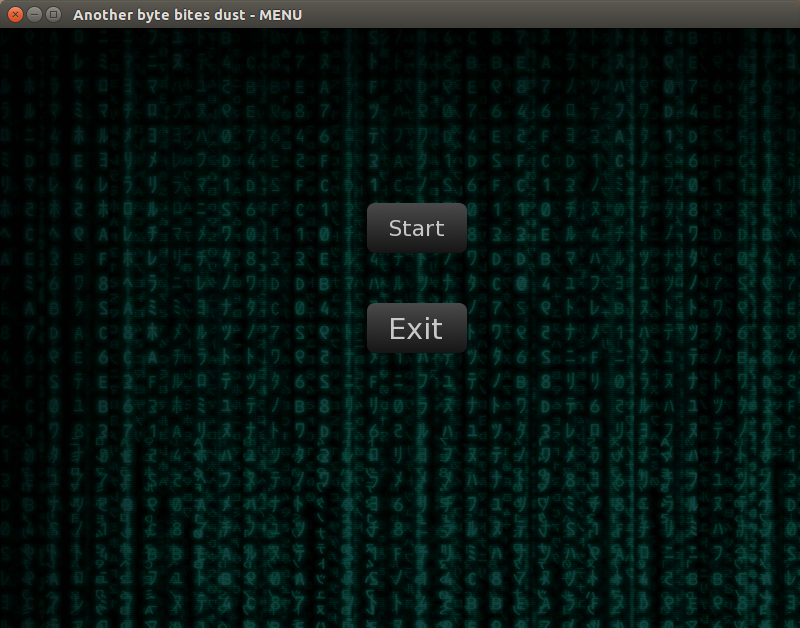
\includegraphics[scale=0.4]{menu.png}
La finestra è creata utilizzando la RenderWindow fornita da SFML.
Il menù contiene una form creata utilizza TGUI la quale contiene i due bottoni start e exit. La form contiene anche l'animazione in background che permette di cambiare sfondo ogni n secondi.
\subsection{Schermata gioco}
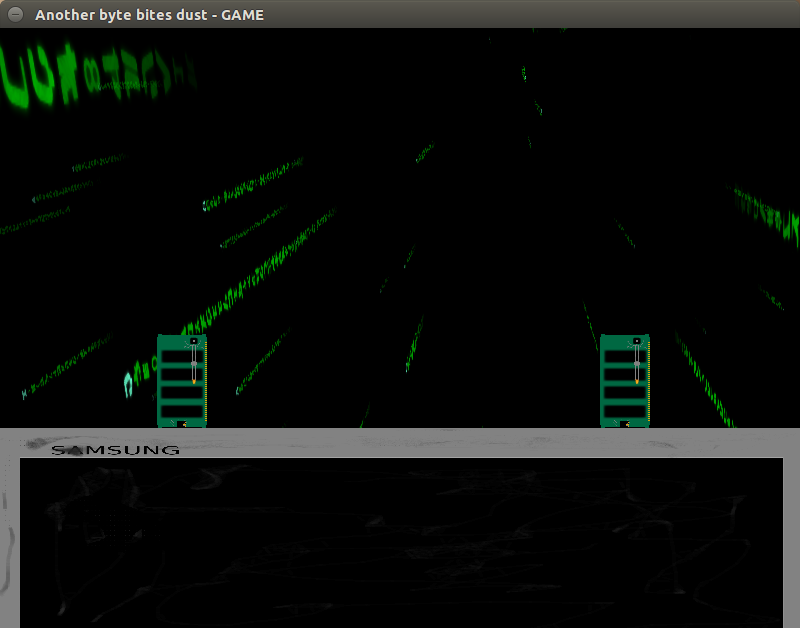
\includegraphics[scale=0.4]{game.png}
Premuto il tasto start la form viene eliminata e si inizializza ogni risorsa utilizzata nel gioco (textures,suoni,immagini).Al caricamento delle risorse il mondo sarà mostrato (monitor o terreno + galassia matrix o sfondo) e i due giocatori (due RAM) cadranno da metà finestra (per mostrare l'implementazione della gravità nel gioco. I due giocatori potranno, attraverso i tasti direzionali (freccie direzionali o WASD) muoversi nel mondo e saltare(sempre prendendo in considerazione la gravità). Al contatto dei due giocatori attraverso attacchi come il pugno o la caduta in volo, uno dei due perdere punti vita e con l'andare dei colpi perderà.
\section{Le difficoltà}
Per quanto il gioco sia teoricamente facile, la sua realizzazione pratica è stata abbastanza studiata.
\subsection{Le animazioni}
Per realizzare le animazioni il programmatore a più metodi a disposizione
\begin{itemize}
\item Creare una immagine(frame) per ogni parte del movimento
\item Creare una sola immagine(sprite) con uno scheletro ed utilizzare le matrici di trasformazione per modificare l'immagine
\item Creare un modello 3D con scheletro e considerare solo due dimensioni
\end{itemize}
La creazione di animazioni non è semplice poichè richiede molto tempo e/o software commerciali da centinaia di euro. La prima opzione si è rivelata la più economica. Ho creato una sprite del giocatore e, partendo da quella, tramite un programma di editing immagine, ho modificato gambe e braccia per n volte, creando una sensazione di movimento.
\subsection{La gestione delle risorse}
Caricare un'immagine è semplice, mentre ottimizzare i tempi di caricamento no. Tramite la libreria Thor ho create un gestore di risorse in grado di caricare delle spritesheet, ovvero una sola immagine contenente più sprite e le loro animazioni. In questo modo, le risorse possono essere condivise da ogni giocatore, senza essere duplicate e soprattutto, caricandole insieme rendono il lavoro della GPU meno pesante.
\subsection{La gravità}
Simulare un salto o una caduta è abbastanza semplice, simulare delle accelerazioni nello spazio e nel tempo un po' di meno. Per rendere il salto credibile bisogna utilizzare teoremi come il metodo di Eulero o l'algoritmo di Størmer-Verlet ed applicarlo al piano del gioco dove 0 non è il centro ma l'ordinata maggiore è l'altezza l'ordinata minore e origine in $\frac{larghezza}{2}$ $\frac{altezza}{2}$
La formula viene descritta nella sottosezione degli fps.
\subsection{La gestione degli fps}
Gli fps(Immagini mostrate dal monitor al secondo) molti meccanismi semplici in meccanismi più complessi: il movimento di un oggetto nel mondo deve essere direttamente proporzionale al tempo tra un frame ed il successivo, complicando le formule utilizzate sia per il movimento che per la gravità.
$posizione (x,y_{corrente})$	\\
$velocit\grave{a} (x, y_{gravit\grave{a}} + y_{impulsi})$\\
$y_{posizione} = y_{posizione} + (y_{velocit\grave{a}} \times \Delta{Secondi})$\\
$y_{velocit\grave{a}} = y_{velocit\grave{a}} + (y_{Accelerazione} \times \Delta{Secondi})$\\
\chapter{Conclusioni}
\section{Conclusioni personali}
Il progetto è stato un grande modo per imparare cose nuove, riguardo alle nuove funzionalità del C++11, l'animazione di un oggetto e la fisica. Utilizzare strumenti commerciali molto utilizzati e conoscerli è molto importante nel mondo del lavoro dove programmare non è solo un file con del codice, ma molto di più. Creare il primo videogioco era un mio obbiettivo da molto tempo ed il prossimo sarà tuffarsi nel mondo dell'intelligenza artificiale, molto probabilmente continuando dove mi son fermato con questo progetto.
\end{document}